\section{Supplemental Results}\label{a:res}
%===================================================================================================
\subsection{Base Case}\label{a:res.bc}
%---------------------------------------------------------------------------------------------------
\subsubsection{Distribution of Infections}\label{a:res.bc.inf}
The following figures explore the numbers and proportions of infections
transmitted between risk groups, stratified by partnership type throughout the epidemic.
For each stratification (from, to, partnership type, and year),
we use the median numbers of infections across all model fits.
Figure~\ref{fig:inf.part} illustrates
infections transmitted via the modelled partnership types over time in the base case, while
Figure~\ref{fig:inf.frto} illustrates
the risk groups transmitting (\subref{fig:inf.fr}) and acquiring (\subref{fig:inf.to}) infections.
Figure~\ref{fig:inf.alluvial} illustrates the distribution of infections
stratified by all three factors every 10 years using an alluvial diagram.
Figure~\ref{fig:inf.ratio} illustrates
the ratio of infections transmitted from vs acquired among individuals in each risk group,
which could be interpreted as a measure related to the group-specific reproductive number.
\begin{figure}[h]
  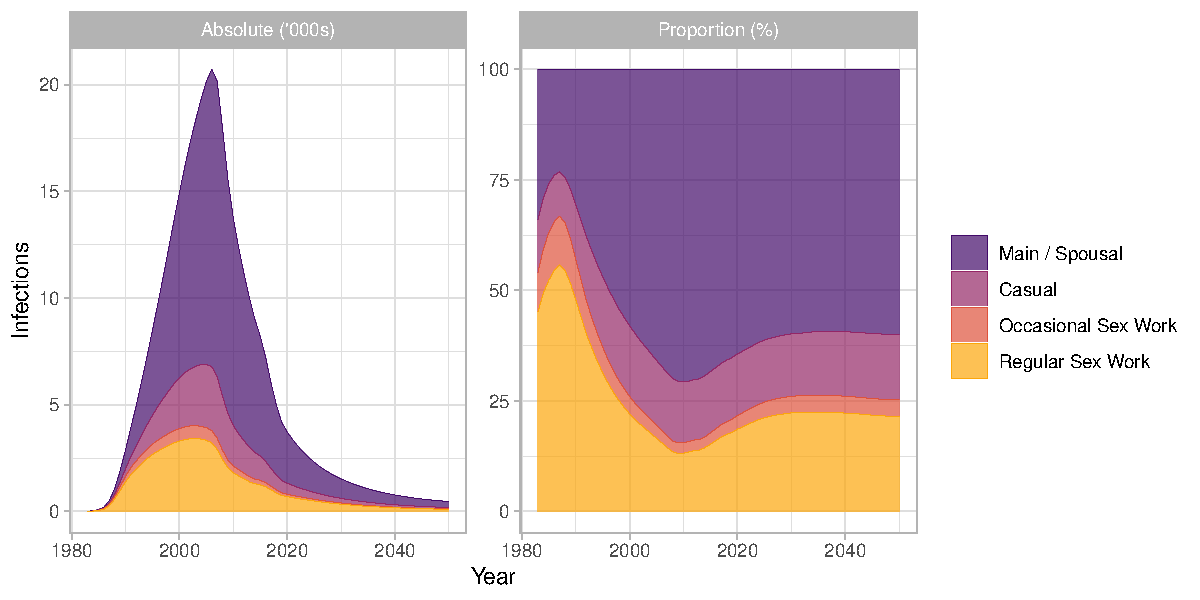
\includegraphics[width=\linewidth]{inf-base-part}
  \caption{Absolute numbers and proportions of infections
    transmitted via different modelled partnership types
    in the base case scenario}
  \label{fig:inf.part}
  \floatfoot{Median numbers of infections across all model fits are shown.}
\end{figure}
\begin{figure}[h]
  \begin{subfigure}{\linewidth}
    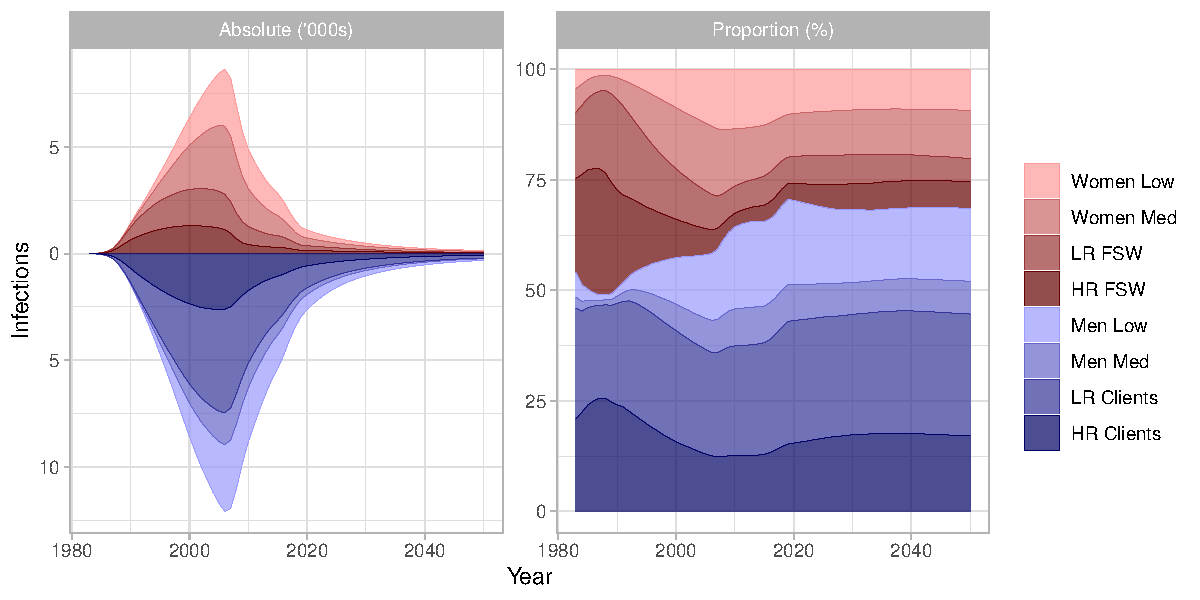
\includegraphics[width=\linewidth]{inf-base-from}
    \caption{Transmitted from}
    \label{fig:inf.fr}
  \end{subfigure}
  \begin{subfigure}{\linewidth}
    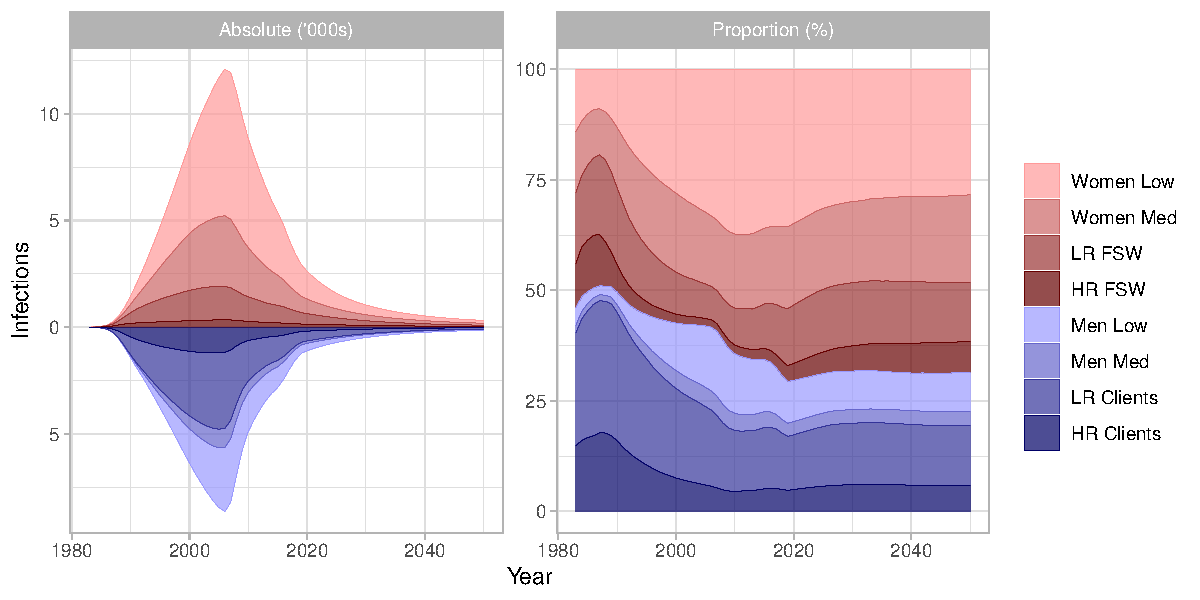
\includegraphics[width=\linewidth]{inf-base-to}
    \caption{Acquired among}
    \label{fig:inf.to}
  \end{subfigure}
  \caption{Absolute numbers and proportions of infections
    (\subref{fig:inf.fr}) transmitted from and (\subref{fig:inf.to}) acquired among modelled risk groups
    in the base case scenario}
  \label{fig:inf.frto}
  \floatfoot{Notation ---
    Low/LR: lower risk; Med: medium risk; HR: higher risk; FSW: female sex workers; Clients: of FSW.
    Median numbers of infections across all model fits are shown.}
\end{figure}
\begin{figure}[h]
  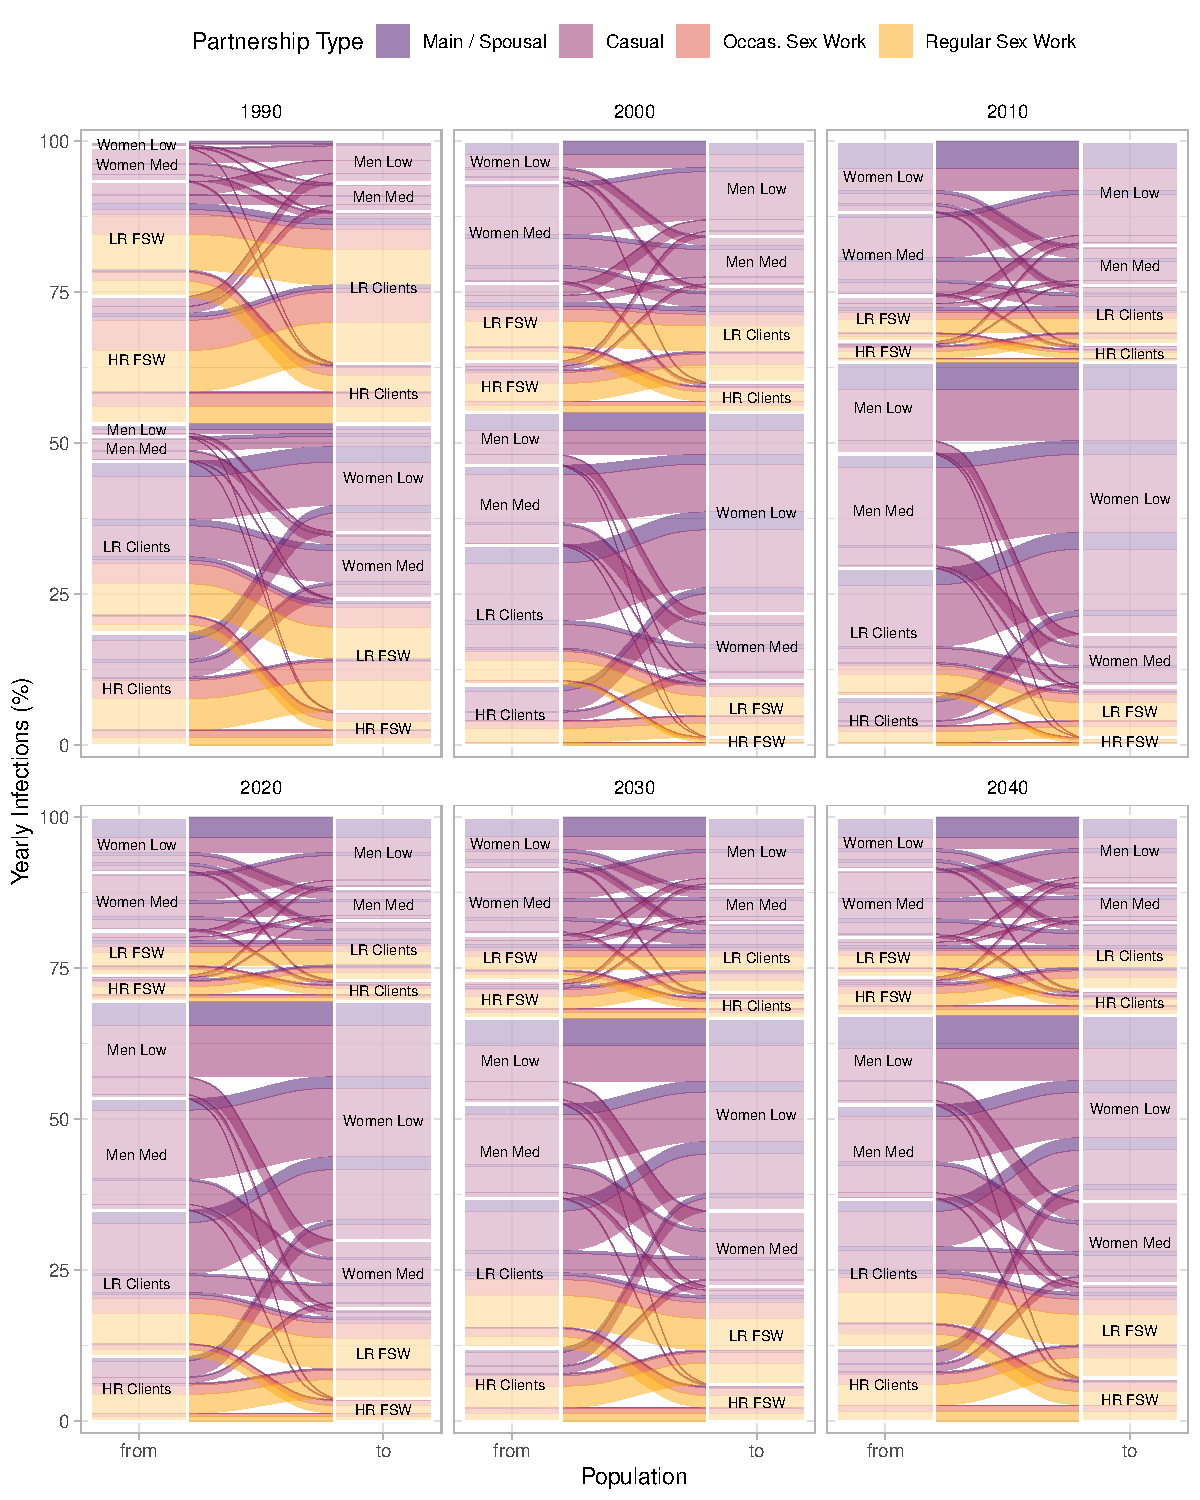
\includegraphics[width=\linewidth]{inf-base-alluvial}
  \caption{Alluvial diagram showing proportions of all yearly infections (flows)
    transmitted from (left) to (right) modelled risk groups,
    stratified by partnership type (color) and year (facets),
    in the base case scenario}
  \label{fig:inf.alluvial}
  \floatfoot{Median numbers of infections across all model fits are shown.
    An animated version of this figure is available online at
    \hreftt{github.com/mishra-lab/hiv-fsw-art}}
\end{figure}
\begin{figure}[h]
  \centering
  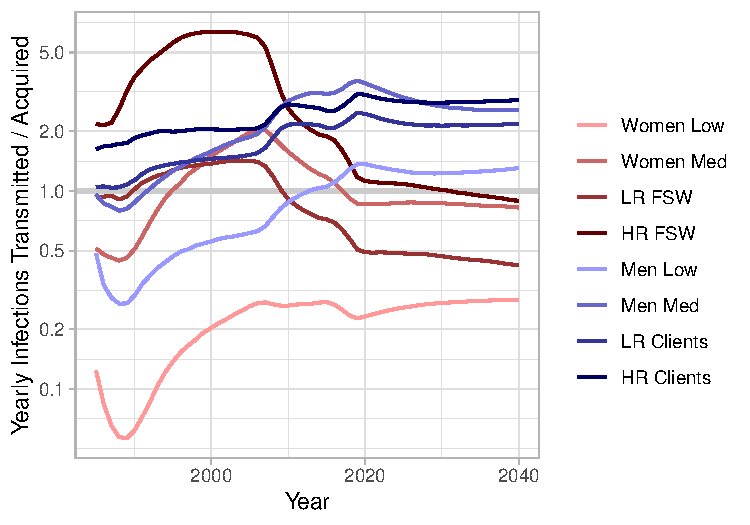
\includegraphics[width=.7\linewidth]{inf-base-ratio}
  \caption{Ratio of yearly infections transmitted from vs acquired among modelled risk groups
    in the base case scenario}
  \label{fig:inf.ratio}
  \floatfoot{Median numbers of infections across all model fits are shown.}
\end{figure}
\clearpage
%===================================================================================================
\subsection{Objective 1}\label{a:res.1}
%---------------------------------------------------------------------------------------------------
\subsubsection{Additional Incidence}
%Figure~\ref{fig:obj.1.inc} illustrates \dots
%\begin{figure}[h]
%  \centerline{\includegraphics[width=\bigfig]{obj_1_inc}}
%  \caption{HIV Incidence in the base case and counterfactual scenarios}
%  \label{fig:obj.1.inc}
%  \floatfoot{Median incidence across all model fits is shown}
%\end{figure}
\par
Figure~\ref{fig:obj.1.inc.add} illustrates \dots
\begin{figure}[h]
  \centering
  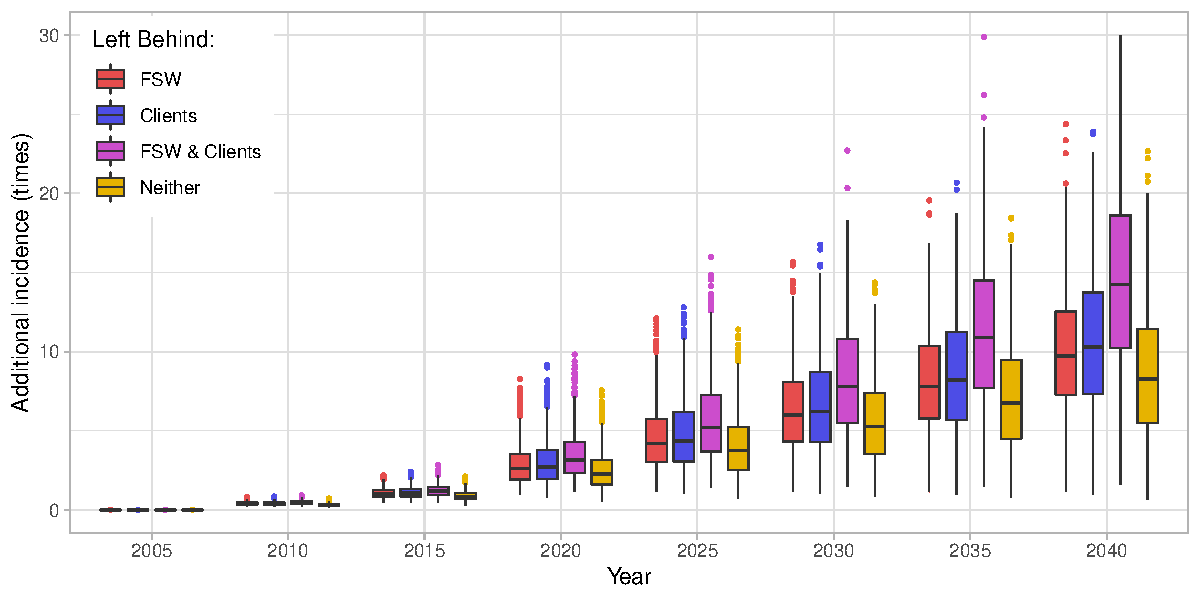
\includegraphics[width=\linewidth]{obj_1_inc_add}
  \caption{Additional HIV incidence (times) in counterfactual scenarios (60-80-80 overall by 2020)
    vs the base case scenario (95-95-95 by 2020).
    Scenarios explore reduced cascades (40-60-80 by 2020) among FSW, clients of FSW, both, or neither
    as part of reduced cascade overall.}
  \label{fig:obj.1.inc.add}
\end{figure}
%---------------------------------------------------------------------------------------------------
\subsubsection{Distribution of Infections}\label{a:res.1.inf}
As in \S~\ref{a:res.bc.inf}, Figure~\ref{fig:inf.diff} illustrates \dots
\begin{figure}[h]
  \begin{subfigure}{\linewidth}
    \centerline{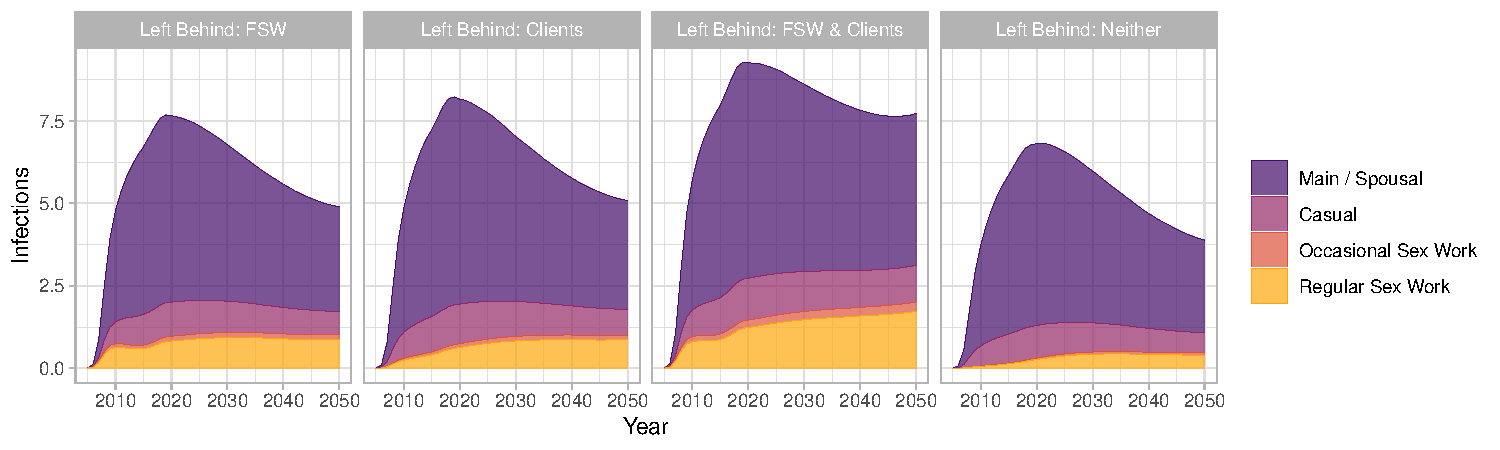
\includegraphics[width=\bigfig]{inf-diff-part}}
    \caption{Partnership type}
    \label{fig:inf.diff.part}
  \end{subfigure}
  \begin{subfigure}{\linewidth}
    \centerline{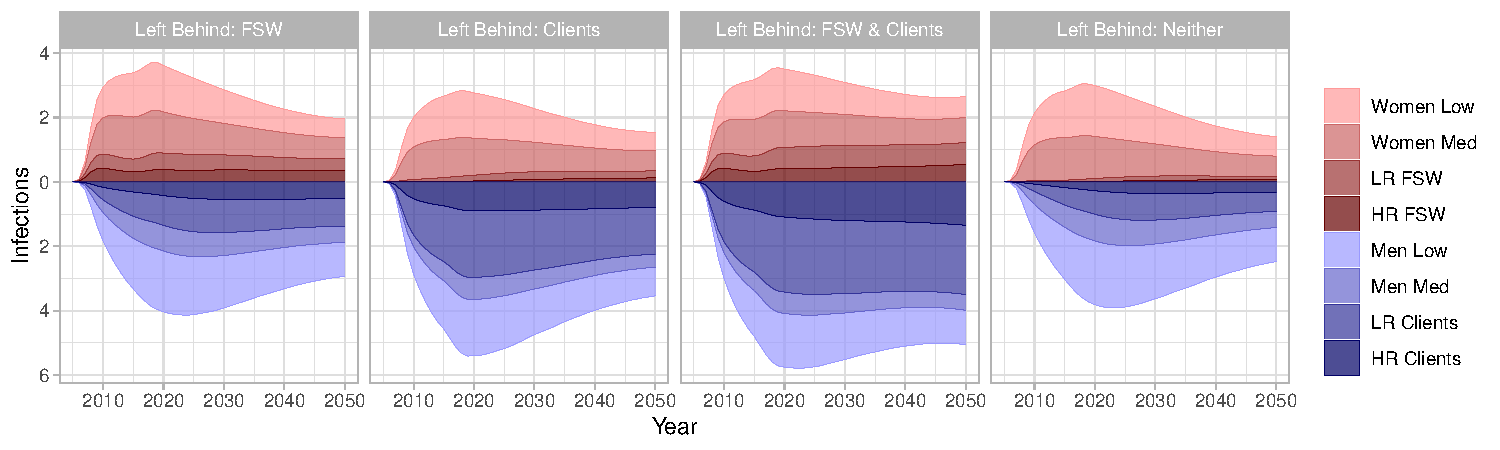
\includegraphics[width=\bigfig]{inf-diff-from}}
    \caption{Transmitted from}
    \label{fig:inf.diff.from}
  \end{subfigure}
  \begin{subfigure}{\linewidth}
    \centerline{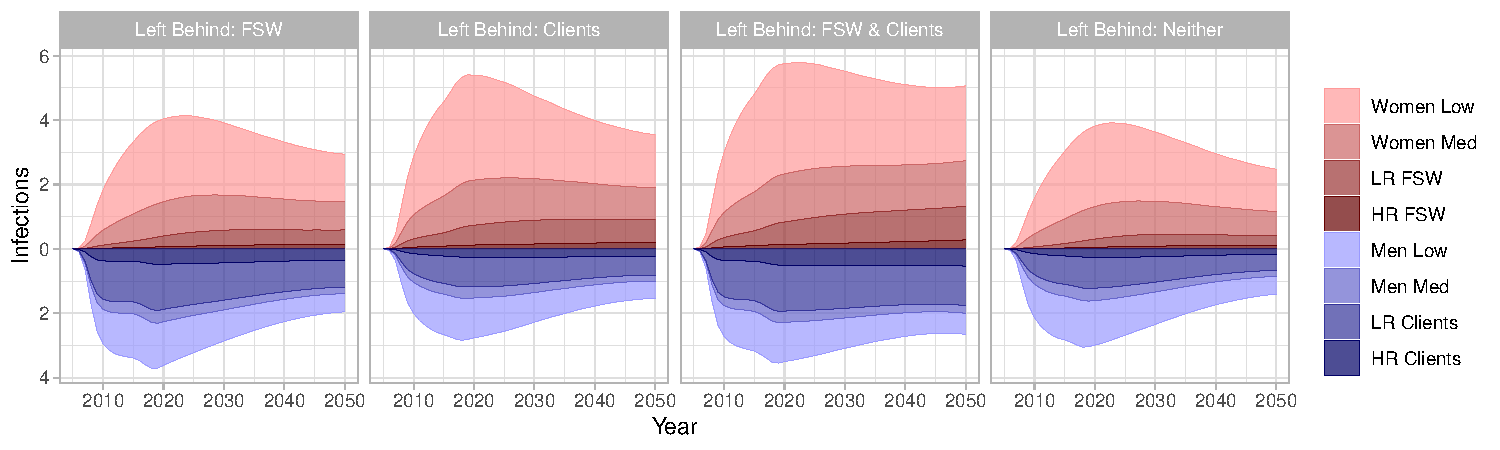
\includegraphics[width=\bigfig]{inf-diff-to}}
    \caption{Acquired among}
    \label{fig:inf.diff.to}
  \end{subfigure}
  \caption{Numbers of additional infections in each counterfactual scenario vs the base case, stratified by:
    (\subref{fig:inf.diff.part}) partnership type,
    (\subref{fig:inf.diff.from}) transmitting group, and
    (\subref{fig:inf.diff.to}) acquiring group}
  \label{fig:inf.diff}
  \floatfoot{Notation ---
    Low/LR: lower risk; Med: medium risk; HR: higher risk; FSW: female sex workers; Clients: of FSW.
    Median numbers of infections across all model fits are shown.}
\end{figure}
\clearpage
%===================================================================================================
\subsection{Objective 2}\label{a:res.2}
Figure~\ref{fig:obj.2.cascade} illustrates
the distribution of HIV treatment cascade attainment by 2020
in randomly sampled scenarios for Objective~\ref{obj:2}, stratified by sub-population.
Median (95\% CI) viral suppression ($VS$) among HIV+ were: % MAN
43~(15,~72)\% among overall,
44~(13,~76)\% among lower risk,
45~(18,~72)\% among FSW, and
33~(9,~65)\% among clients.
\begin{figure}[h]
  \centerline{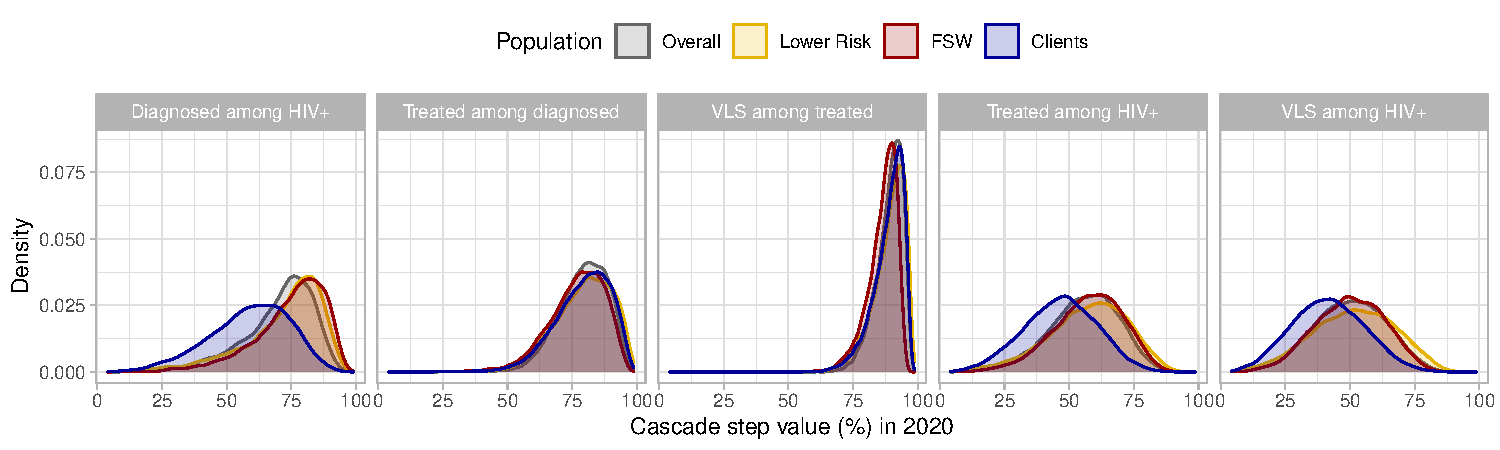
\includegraphics[width=\bigfig]{obj_2_cascade}}
  \caption{Distribution of HIV treatment cascade attainment by 2020
    in randomly sampled scenarios, stratified by sub-population}
  \label{fig:obj.2.cascade}
\end{figure}
\par
Figure~\ref{fig:obj.2.inf.t} expands on Figure~\ref{fig:obj.2.inf}
by illustrating effects over multiple time horizons (2020, 2030, 2040).
Figure~\ref{fig:obj.2.inc} illustrates effects on additional incidence by 2040,
rather than cumulative additional infections.
\begin{figure}
  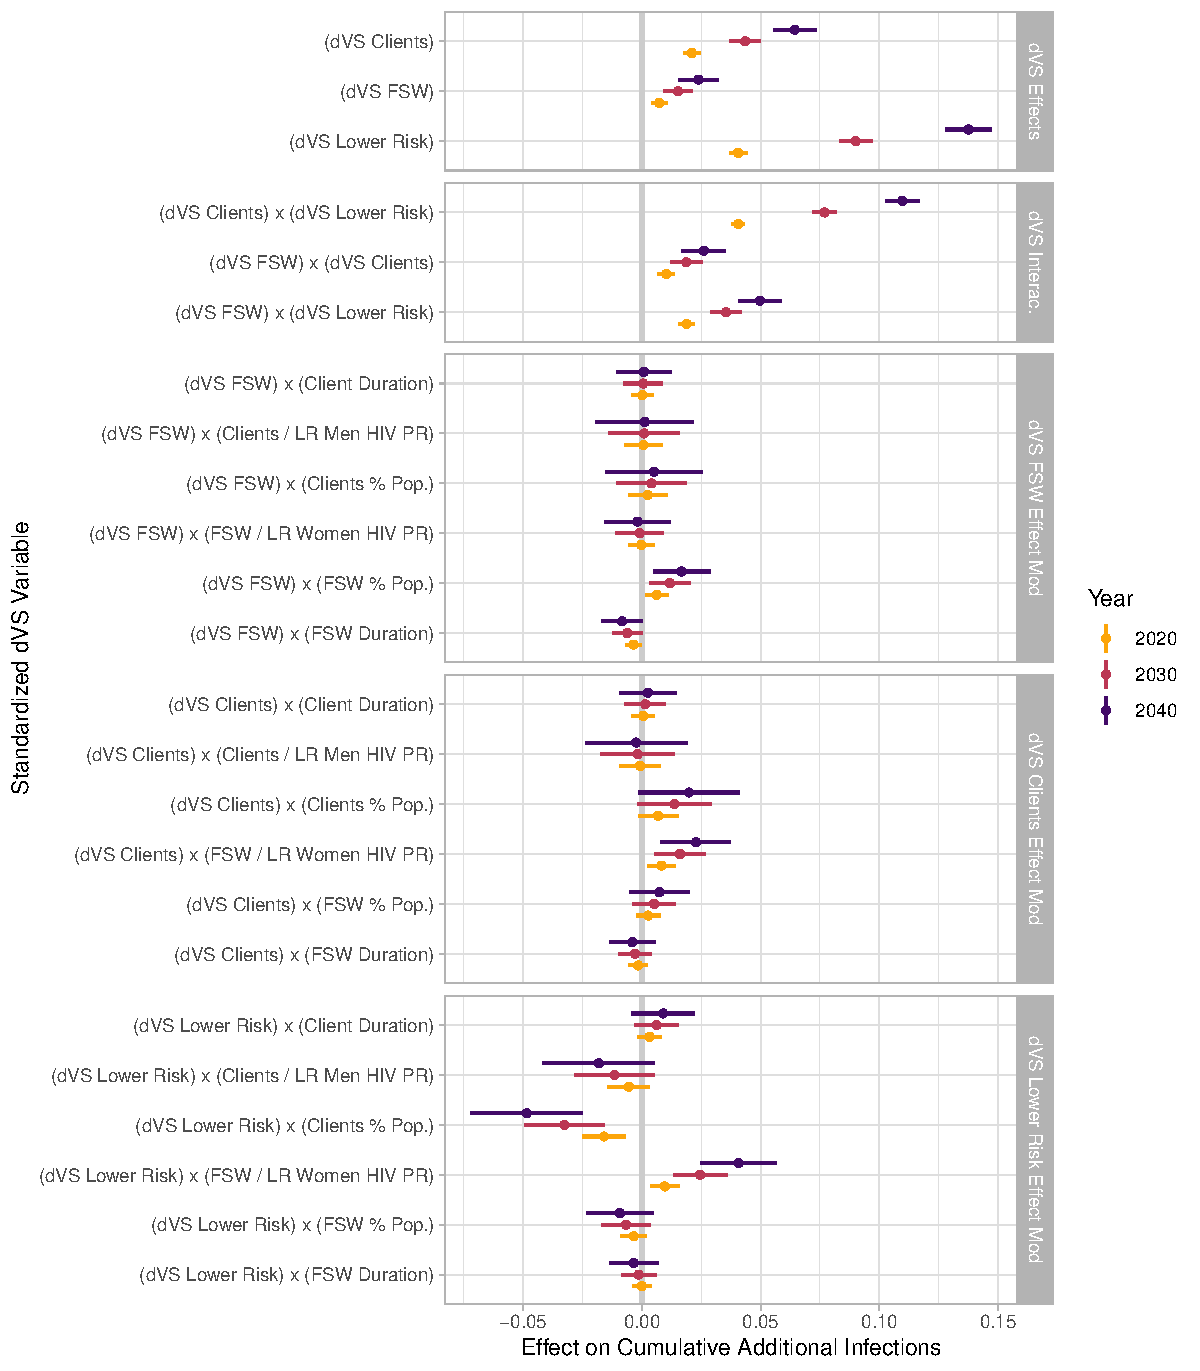
\includegraphics[width=\linewidth]{obj_2_inf_t}
  \caption{Standardized effects of reduced viral suppression ($dVS$) among different populations
    on cumulative additional infections by 2020, 2030, and 2040,
    plus effect modification by epidemic conditions}
  \label{fig:obj.2.inf.t}
  \floatfoot{
    $dVS$: absolute difference in viral suppression in each counterfactual scenario versus the base case;
    FSW: female sex workers;
    Clients: of FSW;
    LR: lower risk;
    Duration: average time spent in the risk group;
    \% Pop: relative population size;
    HIV PR: HIV prevalence ratio.
    All model variables were standardized like
    $\hat{x}_k = (x_k - \mu_{x_k}) / \sigma_{x_k}$
    to reflect the relative influence of variables.}
\end{figure}
\begin{figure}
  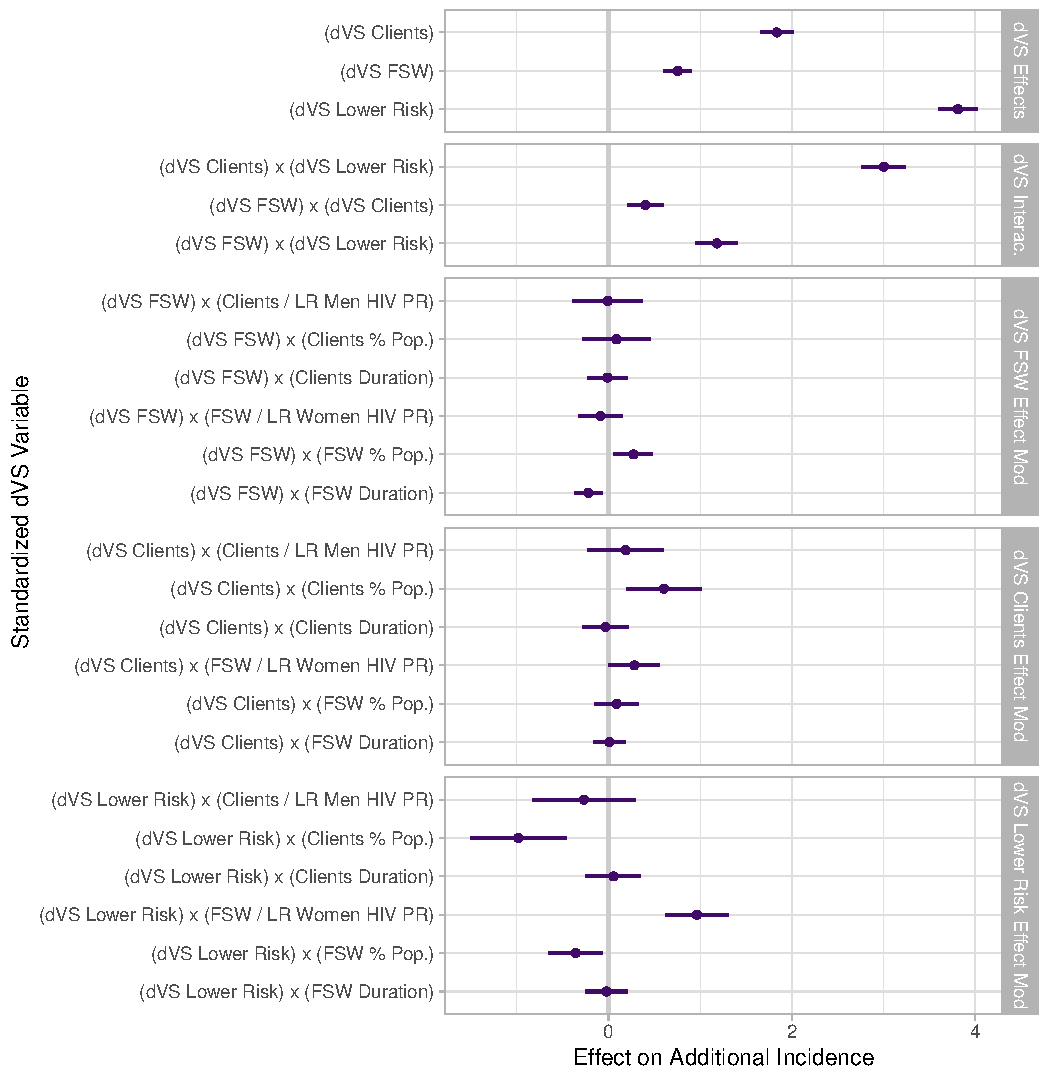
\includegraphics[width=\linewidth]{obj_2_inc}
  \caption{Standardized effects of reduced viral suppression (dVS) among different populations
    on additional incidence by 2040,
    plus effect modification by epidemic conditions}
  \label{fig:obj.2.inc}
  \floatfoot{
    $dVS$: absolute difference in viral suppression in each counterfactual scenario versus the base case;
    FSW: female sex workers;
    Clients: of FSW;
    LR: lower risk;
    Duration: average time spent in the risk group;
    \% Pop: relative population size;
    HIV PR: HIV prevalence ratio.
    All model variables were standardized like
    $\hat{x}_k = (x_k - \mu_{x_k}) / \sigma_{x_k}$
    to reflect the relative influence of variables.}
\end{figure}




